\section{Supplementary Materials}

\subsection{Determining separatrices using the Lande equation}

Under the multivariate breeder's equation \parencite{lande1979quantitative}, evolutionary change in average phenotype $\Delta \bar{z}$ is determined by the amount of standing genetic variation $\mathbf{G}$ and the selection gradient over average fitness $\nabla \ln\ \bar W $:

\begin{equation}
\label{eq:CLT}
\Delta \bar{z}=\mathbf{G}\nabla \ln\ \bar W 
\end{equation}

The adaptive landscapes we treat above define individual fitness, not mean population fitness. To arrive at the mean populaiton fitness, we would need to integrate tover the distribution of phenotypes. If however $Var(z)$ is small relative to the scale of the fitness landscape, higher moments around $\bar{z}$ drop out of the Taylor expansion, and  $\bar{W}\approx W(\bar{z})$. We further need to determine $\mathbf{G}$ in terms of $\mathbf{M}$, which is not possible without accounting for the effect of selection. However, since we start the populations without variation, the G-matrix will be proportional to the M-matrix over the first several generations, which are decisive for the local optimum a population will end up at. Secondly, several theoretical and empirical investigations have shown that $\mathbf{G}$ and $\mathbf{M}$ are often in good alignment with each other \parencite{milocco2022evolution, Houle2017-ph}, as indeed we observe in \FIG[]{fig6}. For the purposes of inferring separatrices through analytical means, we thus assume $\mathbf{G}$ to be proportional to $\mathbf{M}$. We can then use the Lande equation under our two assumptions that $\bar{W}\approx W(\bar{z})$, and that $\mathbf{G} \approx \lambda \mathbf{M}$ to attempt to identify the separatrices deformed by the gene regulatory motifs. The match between these inferred separatrices and the outcomes of our evolutionary simulations is very precise (Supplemental \FIG[]{figS1}, \FIG[]{figS2}), although it mistakenly identifies a separatrix for motifs 1 and 5 in the bottom left of Supplemental \FIG[]{figS1}. The assumptions made above are clearly very simplistic, and we thus do not see this as a result of general relevance. The good match between simulations and analytical inference is to be seen rather to supply a  interpretation of the results of figure 3 rooted in quantitative genetics, that is, seeing the fitness landscape as a gradient field  which is distorted by the shape of heritable genetic variation to yield the evolutionary dynamics.



\begin{landscape}
\begin{figure}[p]
    \centering
    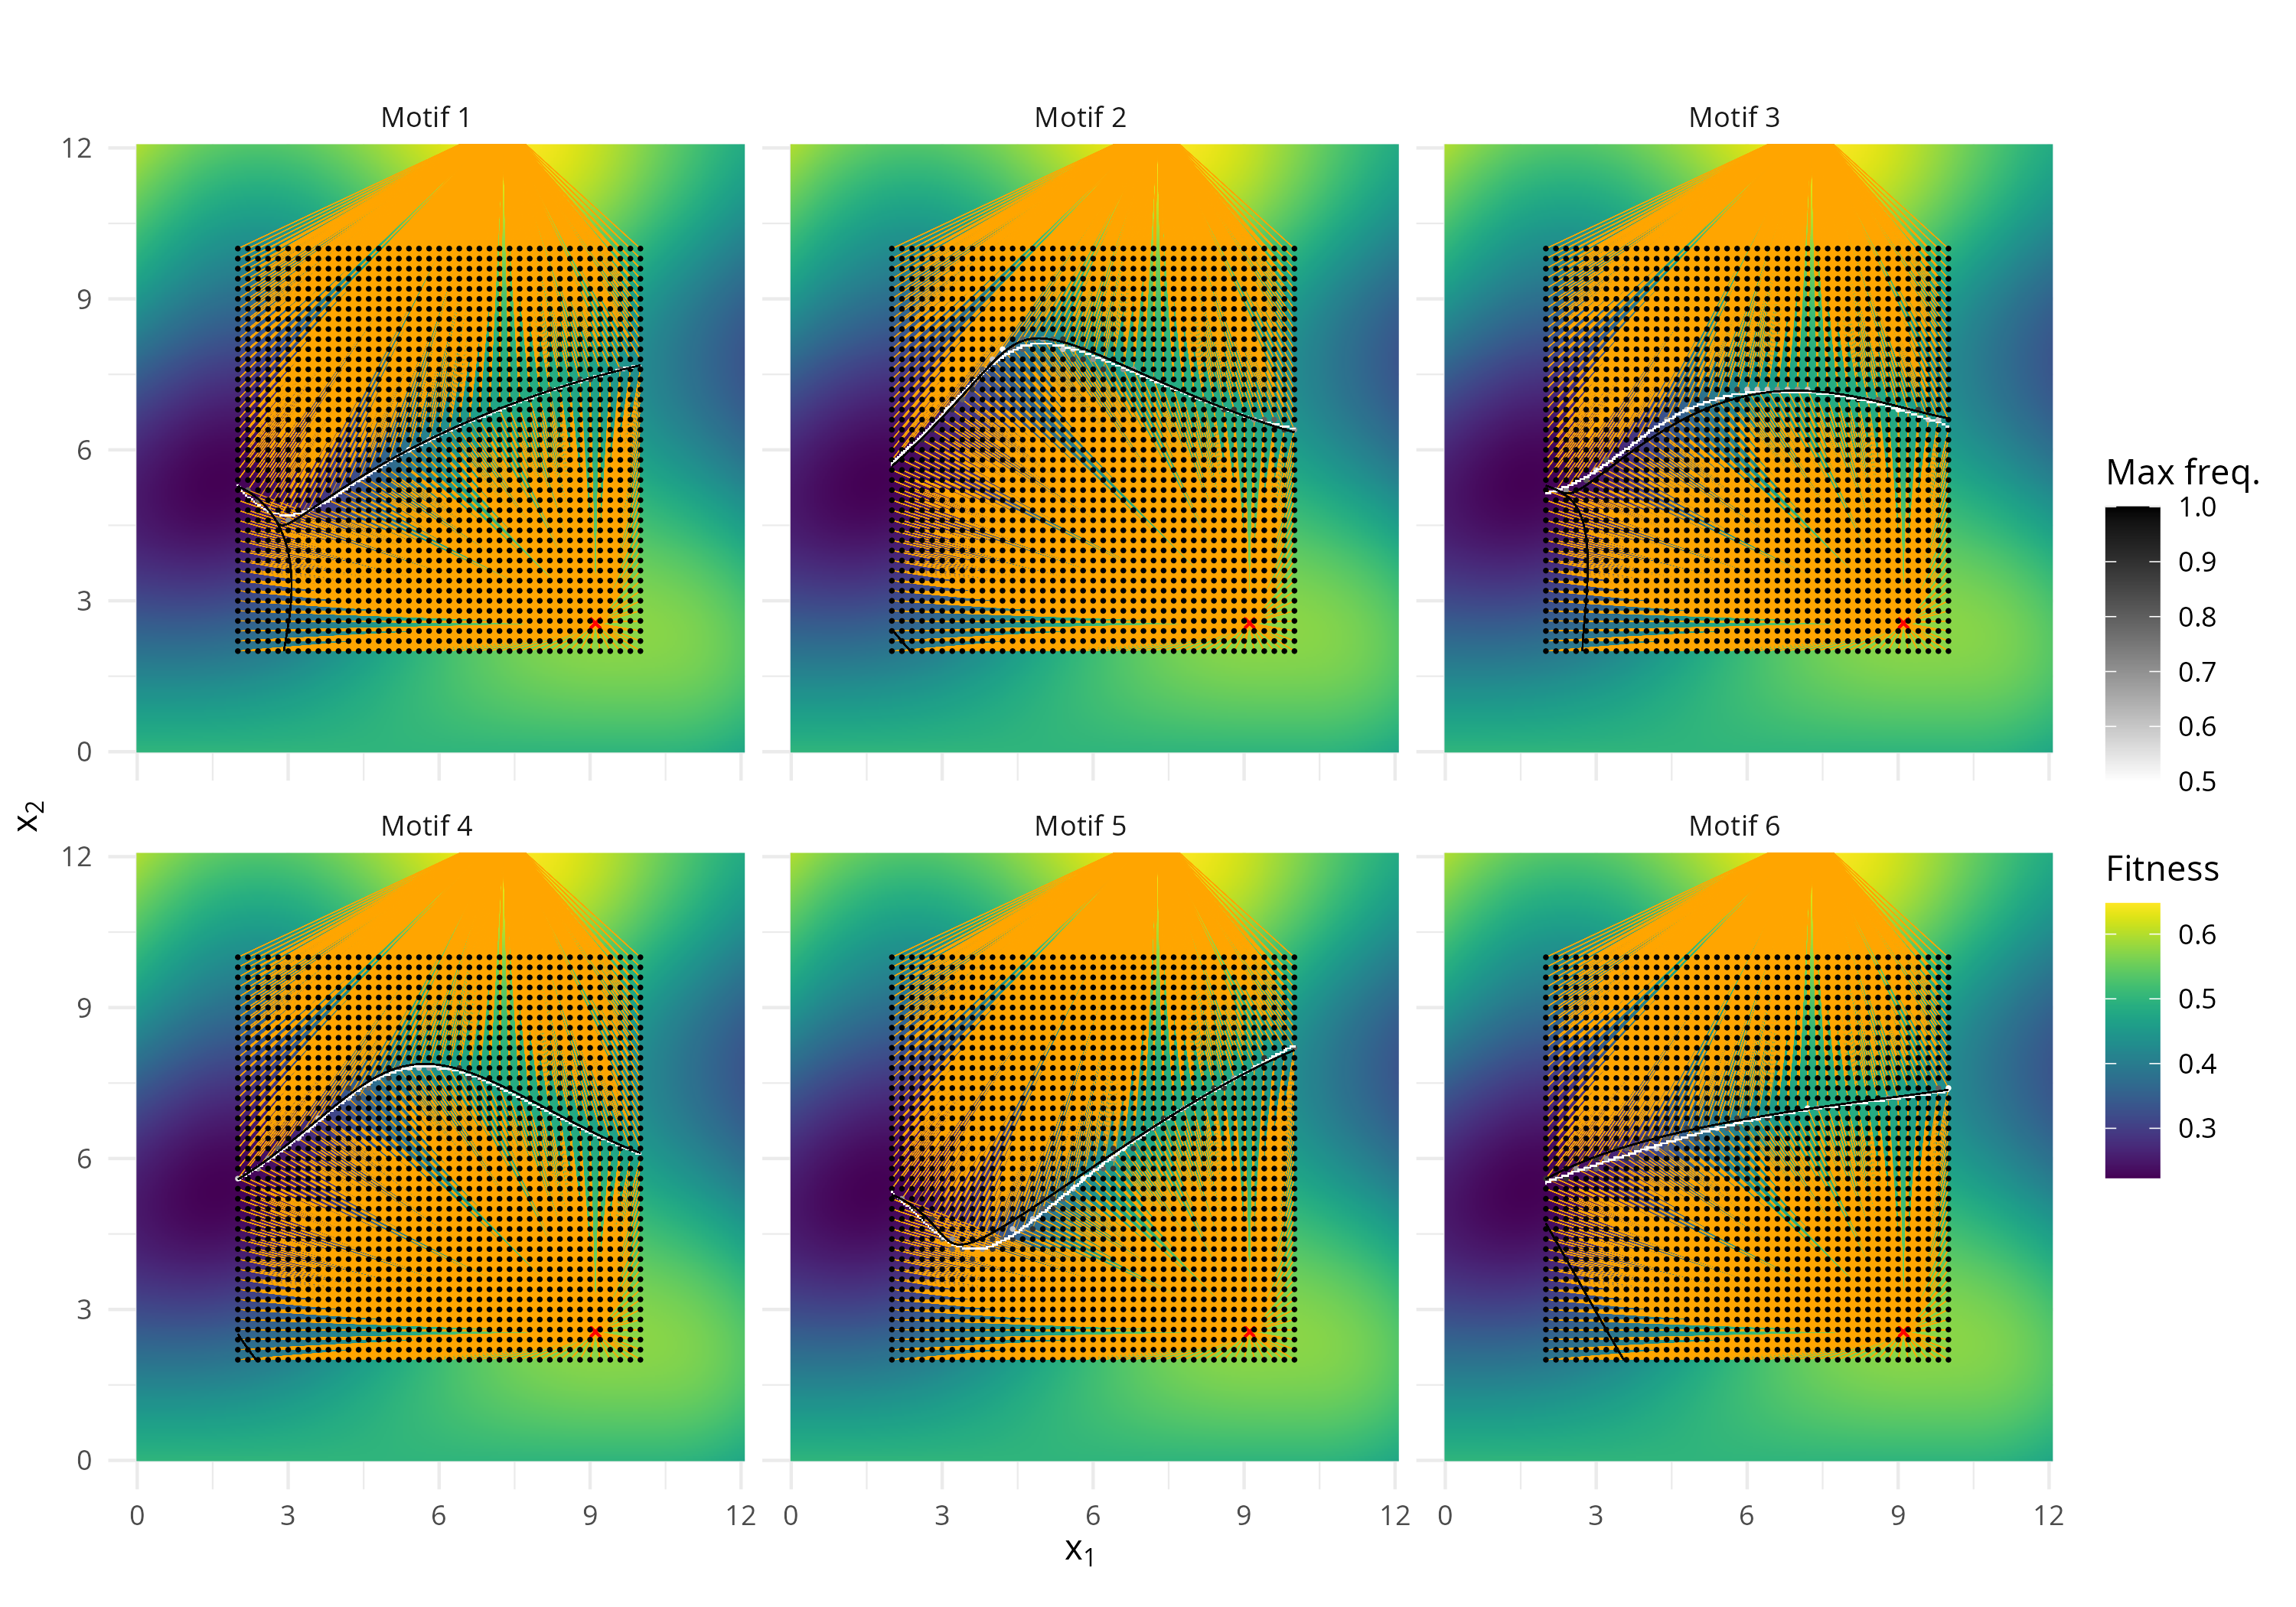
\includegraphics[
        width=\linewidth,
        height=0.9\textheight,
        keepaspectratio
    ]{src/supplementary/figS1.png}
    \caption{\textbf{Evolutionary outcomes on a simple fitness landscape.} We explore a grid of unique starting points, spaced evenly over $x_1, x_2 \in [2, 10]$, and simulate the evolution of 10 replicates over 10,000 generations, or until a local maximum has been reached. Local maxima are highlighted by a red cross, and starting points and outcomes are connected by orange arrows. Starting points are colored with respect to the frequency of the most frequent evolutionary outcome, such that regions of ambiguity show up in white. The observed domains of attraction for each motive as inferred by SVM are delineated in white, the separatrices inferred with the Lande equation are shown in black. The fitness landscape was generated as Perlin noise with a frequency of 0.1. }
    \label{fig:figS1}
\end{figure}

\begin{figure}[p]
    \centering
    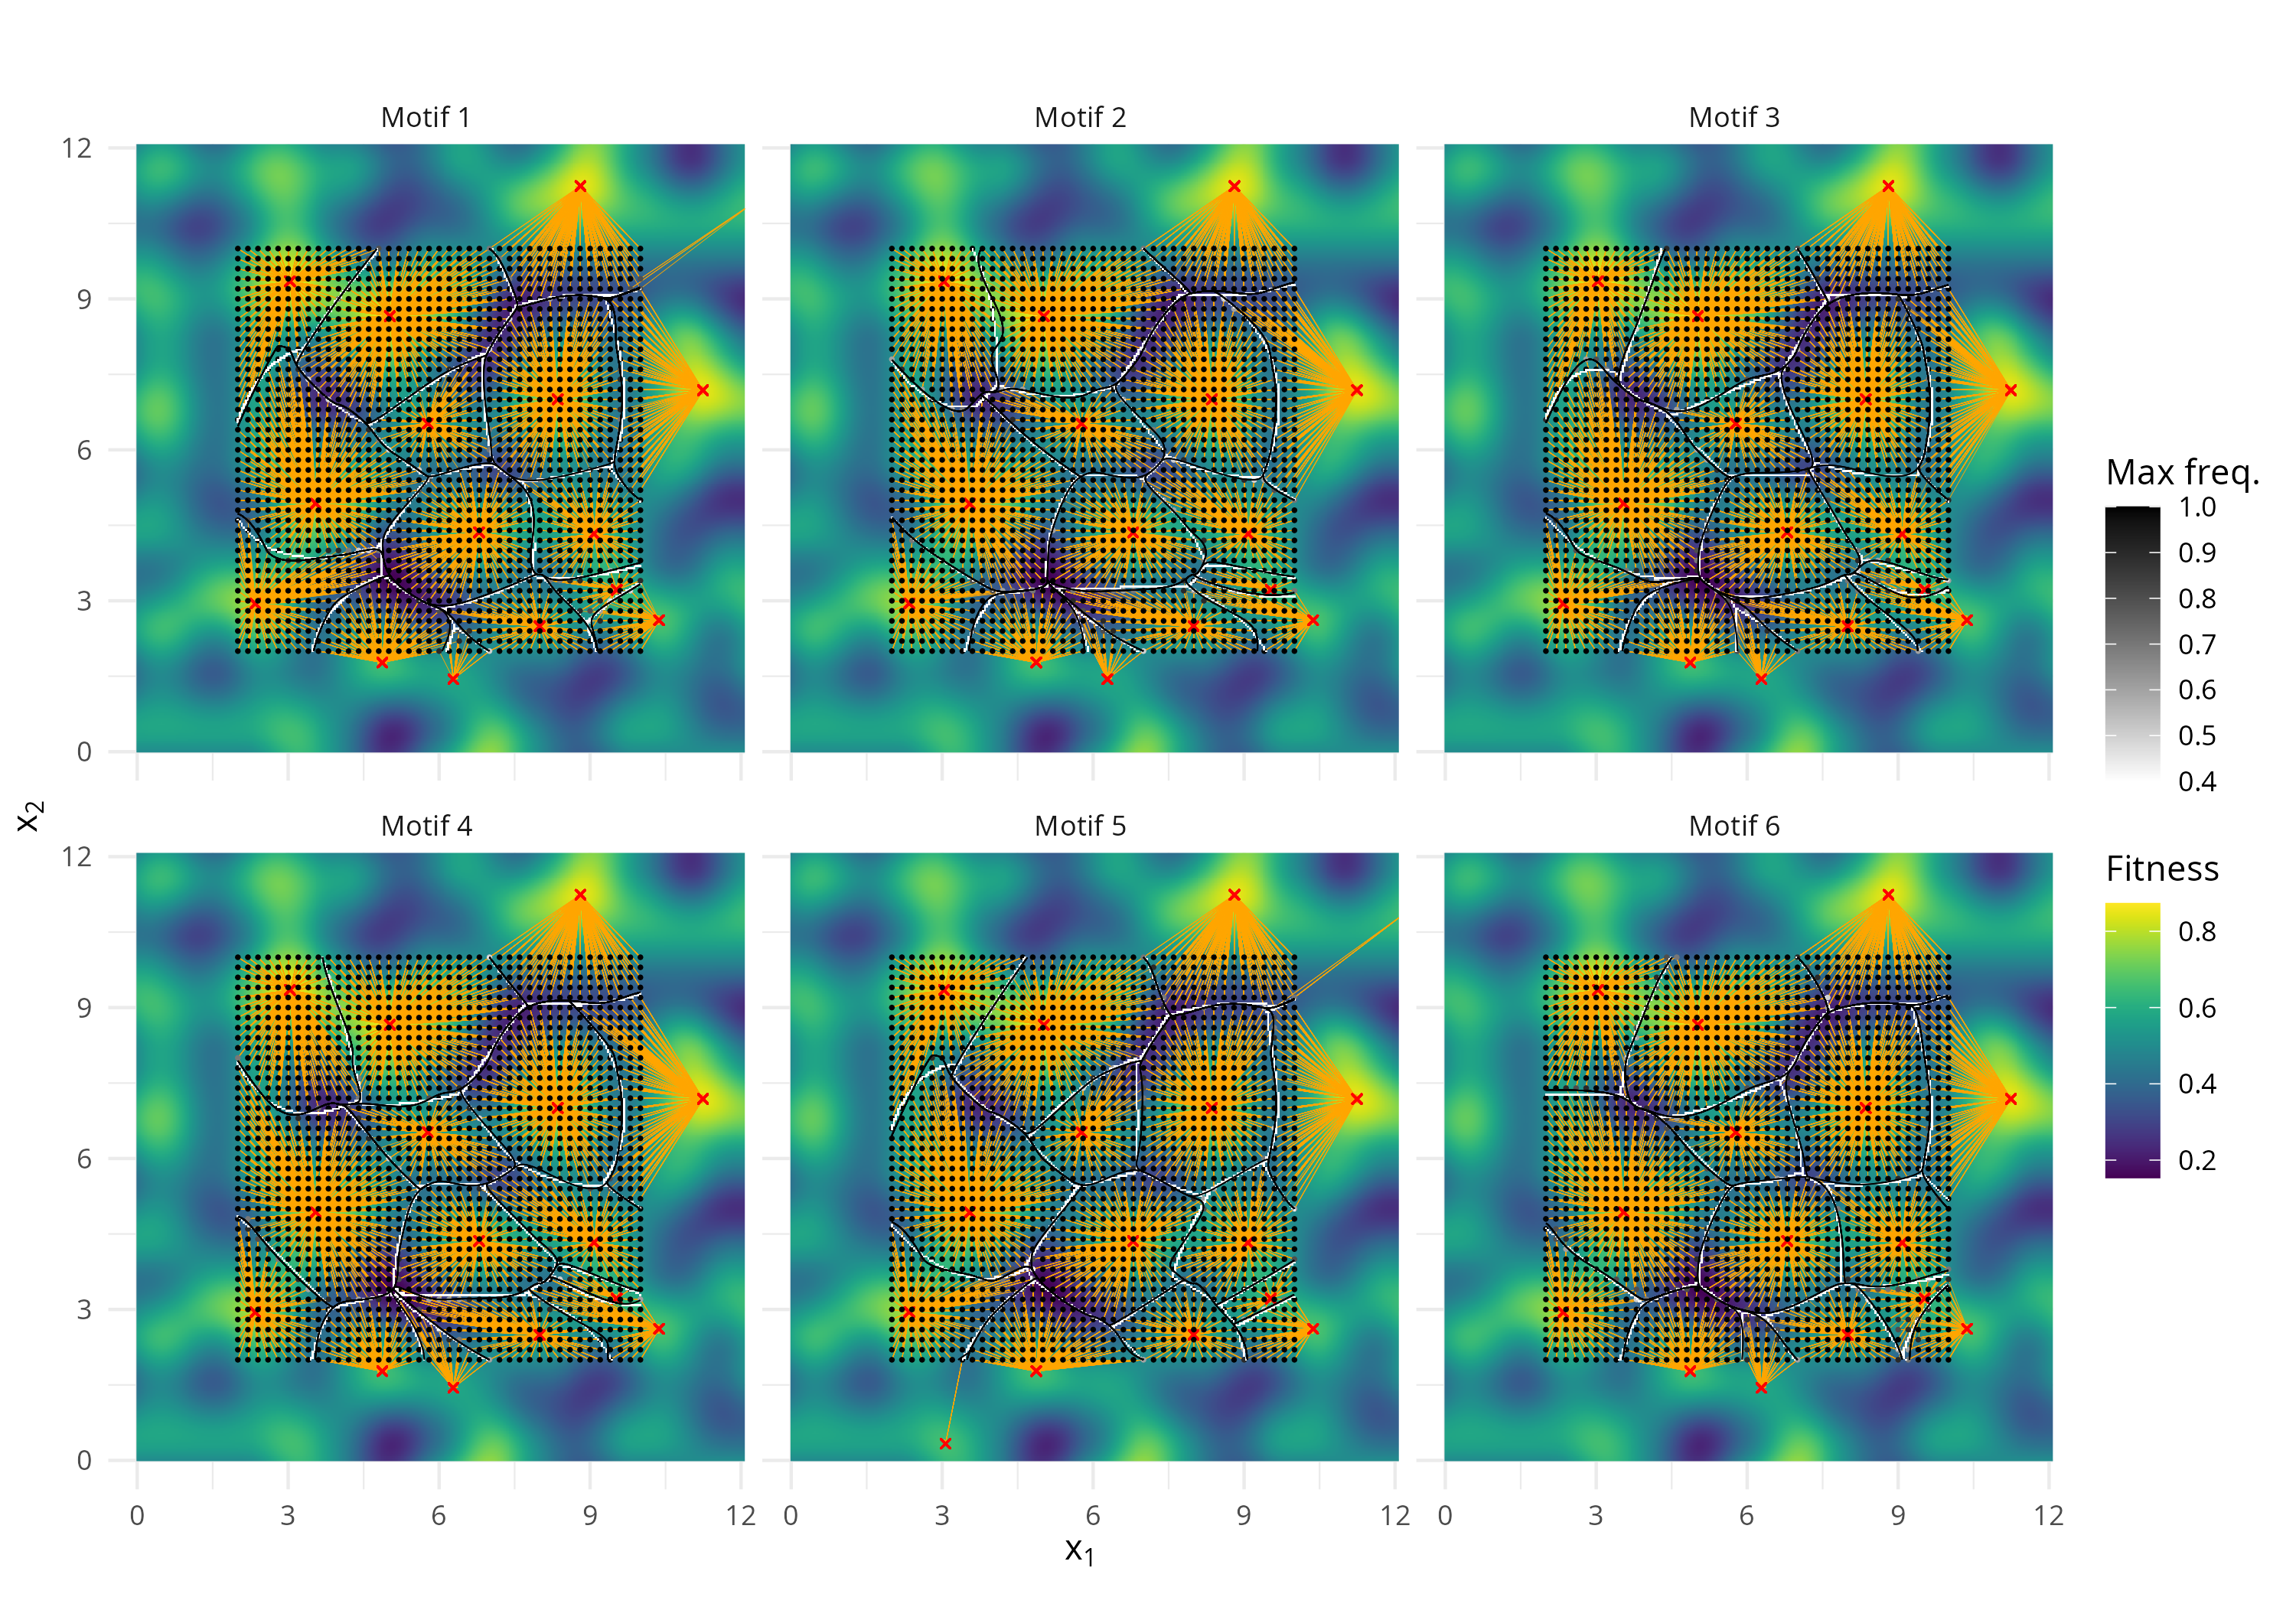
\includegraphics[
        width=\linewidth,
        height=0.9\textheight,
        keepaspectratio
    ]{src/supplementary/figS2.png}
    \caption{\textbf{Evolutionary outcomes on a complex fitness landscape.} We explore a grid of unique starting points, spaced evenly over $x_1, x_2 \in [2, 10]$, and simulate the evolution of 10 replicates over 10,000 generations, or until a local maximum has been reached. Local maxima are highlighted by a red cross, and starting points and outcomes are connected by orange arrows. Starting points are colored with respect to the frequency of the most frequent evolutionary outcome, such that regions of ambiguity show up in white. The observed domains of attraction for each motive as inferred by SVM are delineated in white, the separatrices inferred with the Lande equation are shown in black. The fitness landscape was generated as Perlin noise with a frequency of 0.5. }
    \label{fig:figS2}
\end{figure}
\end{landscape}


\begin{figure}[H]
    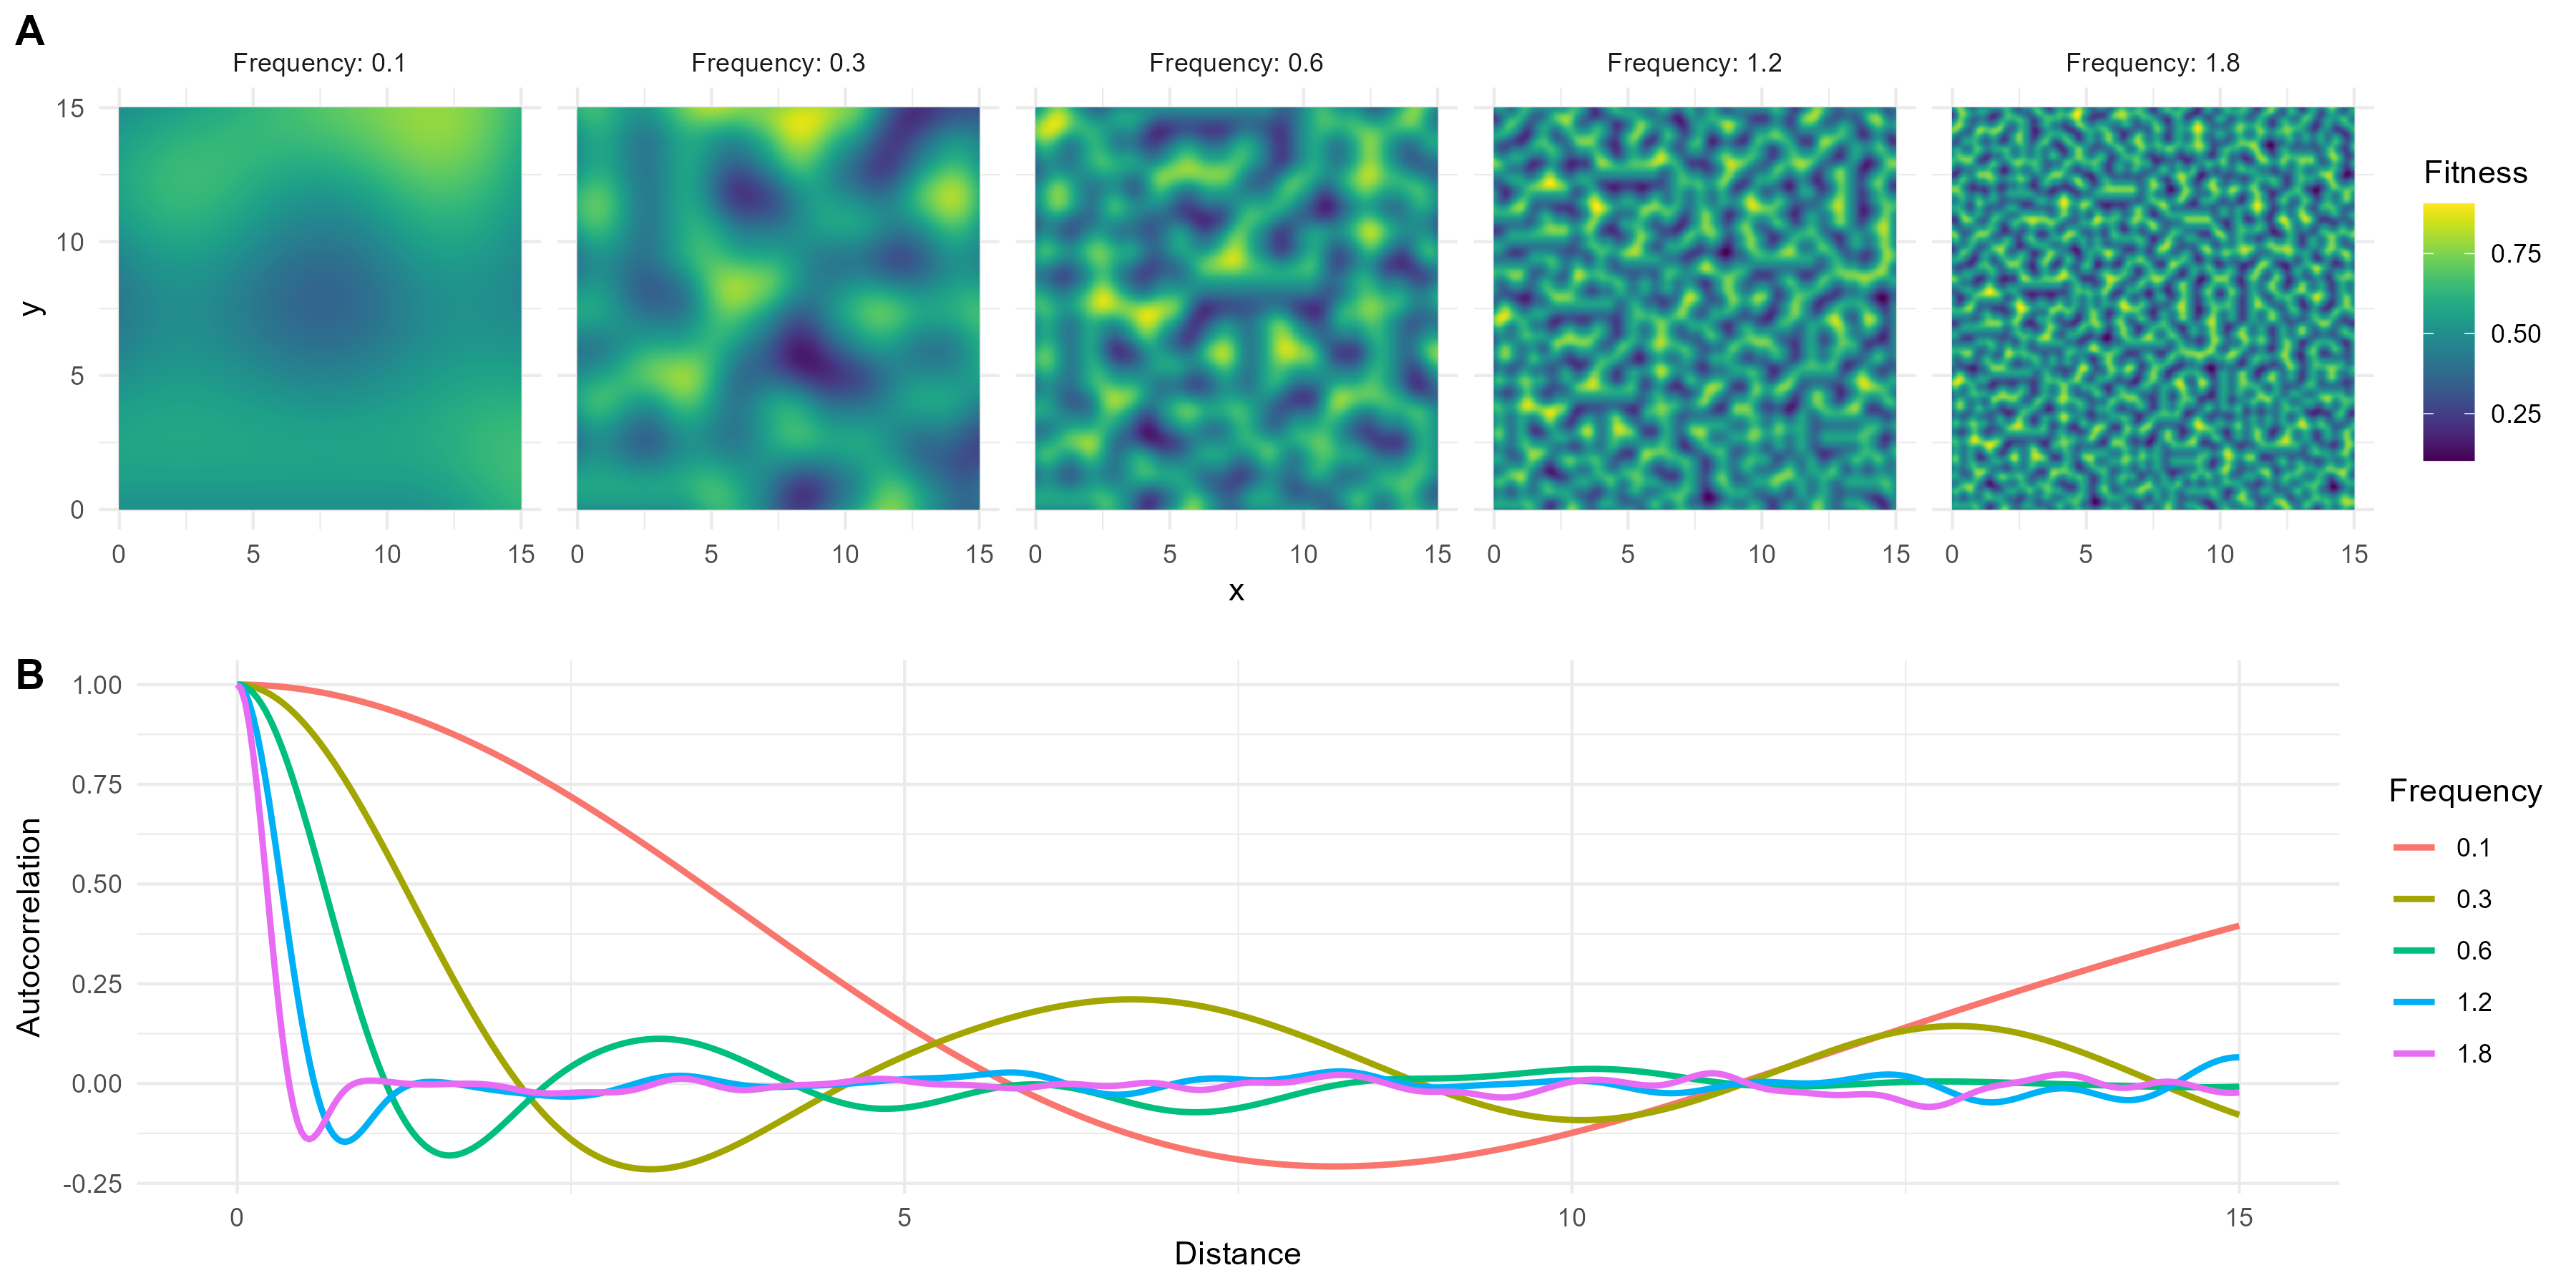
\includegraphics[width=0.65\textheight]{src/supplementary/figS3.png}
    \caption{\textbf{Perlin noise and spatial autocorrelation (A)} Perlin noise of five different frequencies, with identical seeds. \textbf{(B)} Spatial autocorrelation of the plots above. }
    \label{fig:perlin}
\end{figure}